\documentclass[journal,12pt,onecolumn]{IEEEtran}
\usepackage{cite}
\usepackage{amsmath,amssymb,amsfonts,amsthm}
\usepackage{algorithmic}
\usepackage{graphicx}
\usepackage{textcomp}
\usepackage{xcolor}
\usepackage{txfonts}
\usepackage{listings}
\usepackage{enumitem}
\usepackage{mathtools}
\usepackage{gensymb}
\usepackage{comment}
\usepackage[breaklinks=true]{hyperref}
\usepackage{tkz-euclide} 
\usepackage{listings}
\usepackage{gvv}                                        
\def\inputGnumericTable{}                                 
\usepackage[latin1]{inputenc}                                
\usepackage{color}                                            
\usepackage{array}                                            
\usepackage{longtable}                                       
\usepackage{calc}                                             
\usepackage{multirow}                                         
\usepackage{hhline}                                           
\usepackage{ifthen}                                           
\usepackage{lscape}
\usepackage{caption}
\usepackage{subfigure}

% Define \phase command
\newcommand{\phase}[1]{\text{arg}\left(#1\right)}

\newtheorem{theorem}{Theorem}[section]
\newtheorem{problem}{Problem}
\newtheorem{proposition}{Proposition}[section]
\newtheorem{lemma}{Lemma}[section]
\newtheorem{corollary}[theorem]{Corollary}
\newtheorem{example}{Example}[section]
\newtheorem{definition}[problem]{Definition}
\newcommand{\BEQA}{\begin{eqnarray}}
\newcommand{\EEQA}{\end{eqnarray}}
\newcommand{\system}[1]{\stackrel{#1}{\rightarrow}}
\newcommand{\define}{\stackrel{\triangle}{=}}
\theoremstyle{remark}
\newtheorem{rem}{Remark}

\begin{document}

\bibliographystyle{IEEEtran}
\vspace{3cm}

\title{Gate2022.IN.39}
\author{EE22BTECH11008 - Annapureddy Siva Meenakshi$^{*}$}
\maketitle
\bigskip

\renewcommand{\thefigure}{\theenumi}
\renewcommand{\thetable}{\theenumi}
Q: A car is moving collinearly with a laser beam emitted by a transceiver. A laser pulse emitted at $t = 0 \, \text{s}$ is received back by the transceiver $100 \, \text{ns}$ (nanoseconds) later after reflection from the car.A second pulse emitted at  $t = 0.1 \, \text{s}$  is received back  $90 \, \text{ns}$  later. Given the speed of light is $3 \times 10^8 \, \text{m/s}$, the average speed of the
car in this interval is \underline{\quad}.


\solution
\begin{figure}[htb]
  \centering
  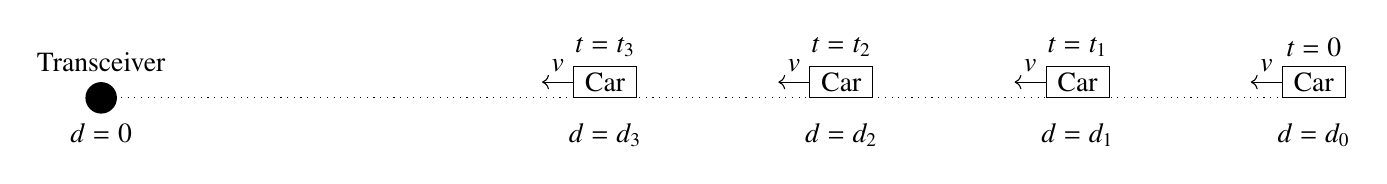
\begin{tikzpicture}

    % Draw the transceiver
    \fill[black] (0,0) circle (0.2) node[above] at (0,0.2) {Transceiver} node[below] at (0,-0.2) {$d=0$};

    % Draw the car at distance D_0
    \draw (15,0) rectangle ++(0.8,0.4) node[midway] {Car} node[above] at (15.4,0.4) {$t=0$ } node[below] at (15.4,-0.2) {$d=d_0$};
    \draw[->] (15,0.2) -- node[above] {$v$} (14.6,0.2);

    \draw (12,0) rectangle ++(0.8,0.4) node[midway] {Car} node[above] at (12.4,0.4) {$t=t_1$ } node[below] at (12.4,-0.2) {$d=d_1$};
    \draw[->] (12,0.2) -- node[above] {$v$} (11.6,0.2);

    \draw (9,0) rectangle ++(0.8,0.4) node[midway] {Car} node[above] at (9.4,0.4) {$t=t_2$ } node[below] at (9.4,-0.2) {$d=d_2$};
    \draw[->] (9,0.2) -- node[above] {$v$} (8.6,0.2);

    \draw (6,0) rectangle ++(0.8,0.4) node[midway] {Car} node[above] at (6.4,0.4) {$t=t_3$ } node[below] at (6.4,-0.2) {$d=d_3$};
    \draw[->] (6,0.2) -- node[above] {$v$} (5.6,0.2);

    \draw[dotted] (0,0) -- (15,0);

\end{tikzpicture}




   \captionsetup{justification=centering, singlelinecheck=off}
  \caption{block diagram of the system}
  \label{fig:EE_58_f1}
\end{figure}

\begin{table}[!ht]
    \centering
        \begin{tabular}{|c|c|c|}
    \hline
    \textbf{Variable} & \textbf{Description} & \textbf{Value} \\
    \hline
    $v_c$ & velocity of laser & $3 \times 10^{8} \, \text{m/s}$ \\
    \hline
    $v$ & average speed of car & none \\
    \hline
    $t_1$ & time at which first pulse hits car & none \\
    \hline
     $t_2$ & time at which second pulse is emmited & $0.1\text{s}$ \\
    \hline
     $t_3$ & time at which  second pulse hits car & none \\
    \hline
    $d_0$  & Distance between tranceiver and car at $t=0$ & none \\
    \hline
    $d_i$ for $i=1,2,3$ & Distance between tranceiver and car at $t=t_i$ & none \\
    \hline
  \end{tabular}


    \caption{Input parameters}
    \label{tab:IN_39_t1}
\end{table}

From ~\figref{fig:EE_58_f1}
\begin{align}
    t_1&=\frac{d_1}{v_c}=\frac{d_0-d_1}{v}\\
\implies d_1&=\frac{d_0}{\left(1+\frac{v}{v_c}\right)}
\end{align}
Distance travelled by first pulse is given by 
\begin{align}
    2d_1 &= v_c \times 100 \, \text{ns}\\
    2\frac{d_0}{\left(1+\frac{v}{v_c}\right)}&=v_c \times 100 \, \text{ns}
    \label{eq:IN.39.4}
\end{align}
similarly time taken by car to move from $d_2$ to $d_3$ is given by
\begin{align}
    t_3-t_2&=\frac{d_3}{v_c}=\frac{d_2-d_3}{v}\\
    \implies d_3&=\frac{d_2}{\left(1+\frac{v}{v_c}\right)}
\end{align}
from ~\figref{fig:EE_58_f1}
\begin{align}
    d_2&=d_0-0.1v\\
\therefore d_3&=\frac{d_0-0.1v}{\left(1+\frac{v}{v_c}\right)}
\end{align}
Distance travelled by second pulse is given by 
\begin{align}
    2d_3 &= v_c \times 90 \, \text{ns}\\
    2\frac{d_0-0.1v}{\left(1+\frac{v}{v_c}\right)}&= v_c \times 90 \, \text{ns} \label{eq:IN.39.10}
\end{align}
solving ~\eqref{eq:IN.39.4} and ~\eqref{eq:IN.39.10} we get

\begin{align}
    v &= 15\, \text{m/s} \\
    v &=54\, \text{Km hr}
\end{align}
\end{document}
